\section{Problem}

Publish-subscribe model is often used in mobile applications to achieve scalable and efficient dispatching of data and notifications between the back-end infrastructure and the mobile applications. Mobile phone data usage is often metered and the bandwidth available in rural areas are often limited compared to cities. SSPS can be seen as a solution to reduce bandwidth usage and thereby, help in cost reduction. However, as of now, there exists no mobile application that uses the SSPS model. Thus, it is not possible to demonstrate the effect of SSPS model for mobile applications dealing with different data formats such as JSON, XML, and CSV.

Additionally, there exists another problem related to the current implementation of the SSPS model. Centralized systems, as the name suggests, are systems where one primary system manages all computing resources. In spite of the benefits of centralized systems such as, small capital and operational cost (minimum hardware), these systems are often faced with problems like single point failure, limited scalability, computational bottleneck, fault tolerance and so on. Thus centralized systems are unsuitable for many large-scale real world applications \parencite{tanenbaum2007distributed}.

In the Simple Shared Dictionary Compression for Publisher-Subscriber (SSPS) model, the entity, Sampling Broker (SB) is responsible for sampling notifications to create, maintain and spread the dictionary to the publishers and subscribers \parencite{Doblander:2016:SDC}. The current implementation of SSPS is on one centralized broker called Moquette \parencite{moquette}. However, one of the major drawbacks is that this sampling broker is a centralized entity and hence it is prone to all the disadvantages of a centralized system.

\makeatletter
\setlength{\@fptop}{0pt}
\makeatother

\begin{figure}[t!]
\centering
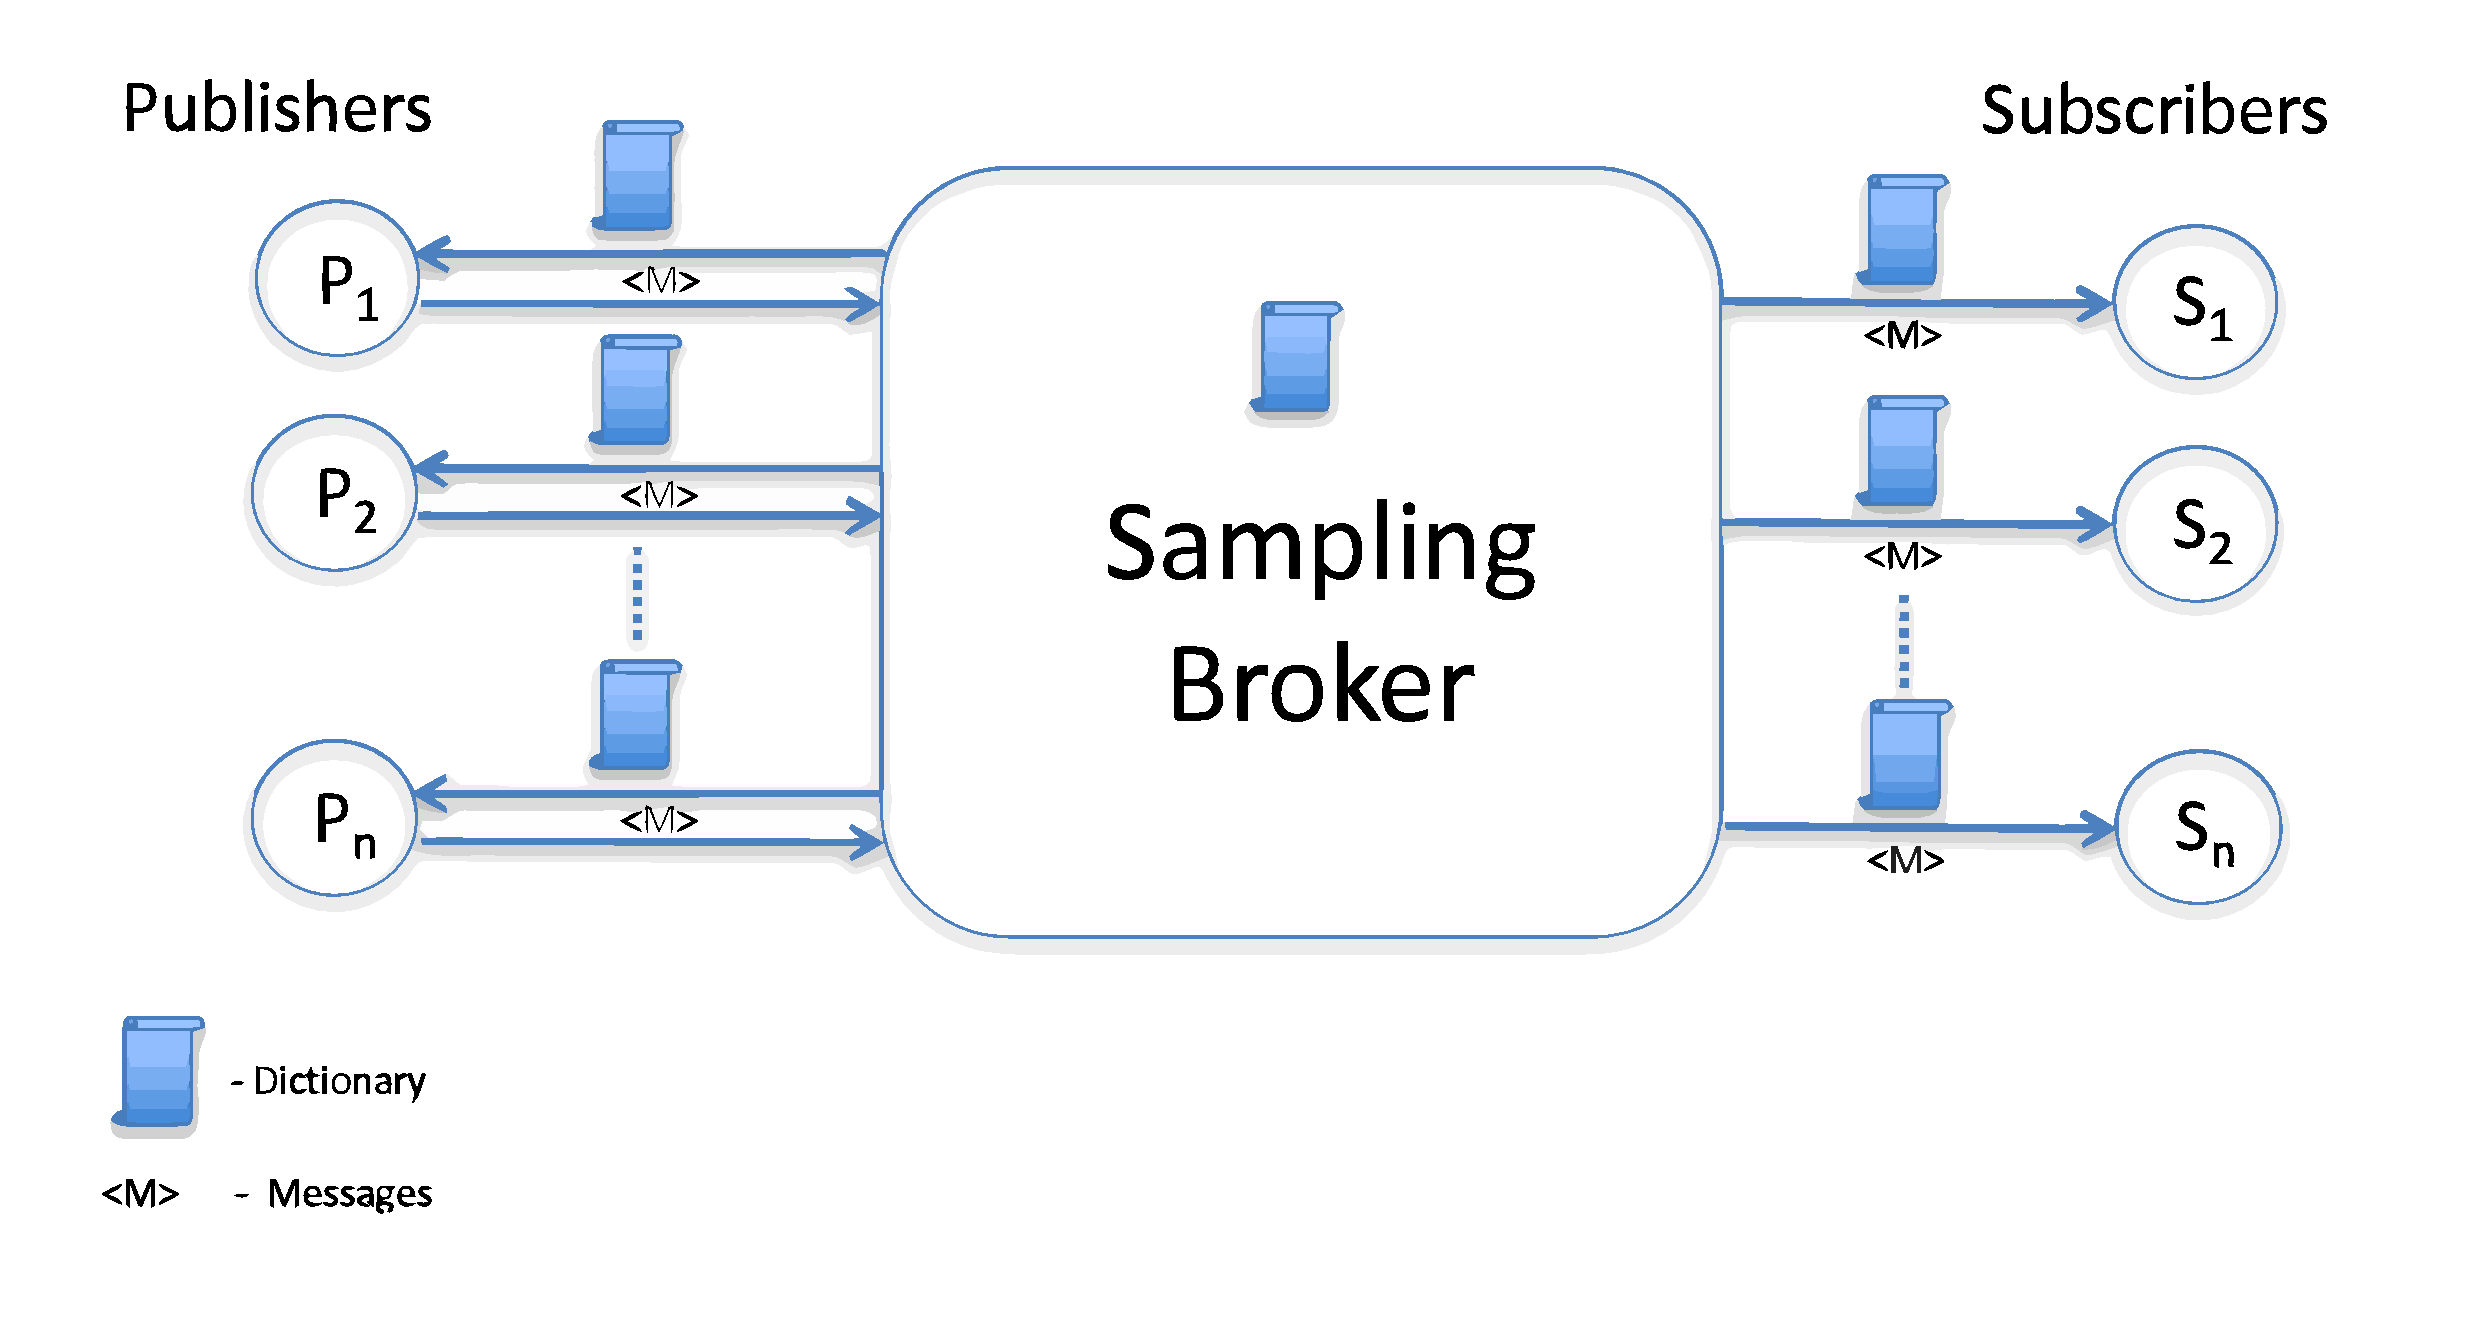
\includegraphics[keepaspectratio, width=.9\textwidth, trim={0 12cm 0 9cm},clip]{ssps.pdf}
\caption{Sampling Broker in SSPS model}\label{figures:ssps}
\end{figure}

Figure \ref{figures:ssps} depicts the state of the art implementation of the SSPS model. As the number of publishers and subscribers increase, there will be a computational bottleneck. Also in a case of failure, the entire SSPS model would collapse, which is not desirable in the real world. Thus, it is needed to overcome the problem of the centralized entity.